\section{Experiments}
\label{sec:experiments}

In this section, we evualuate the core components of \CRATE both individually
and together. It aims to
\begin{enumerate}[leftmargin=*]
\item Validate the space complexity of \LSEQ and highlight the improvement
  over the state-of-the-art.
\item Validate the adaptiveness of \SPRAY, i.e., it automatically resizes the
  neigbhorhood of peers to follow a logarithmic growth compared to the editing
  session membership.
\item Show that \CRATE scales with respect to the number of
  collaborators simultaneously involved in a document editing.
\item Show that concurrency does not impact the size of
  identifiers. Consequently, the space complexity of the identifiers can be
  studies in scenarios without concurrency.
\end{enumerate}

\subsection{CRATE}
\label{subsec:crdt}
\CRATE (CollaboRATive Editor) is a prototype of decentralised editor. We
assume that collaborators can join the document editing and leave when they
want. The group of collaborators can be seen as a peer-to-per network. Hence,
\CRATE uses a gossip dissemination protocol to scale with respect to the
number of collaborators/peers involved in the authoring. In this protocol, each
peer has a set of neighbours and communicates with them. When a peer performs
an operation, it creates a message containing the result of the operation. Each
peer broadcasts its messages and when a peer receives a specific message for
the first time, it re-broadcasts this message. However,
Section~\ref{sec:preliminaries} states that strong eventual consistency is
ensured upon the assumption of eventual delivery, and unfortunately, the
gossiping broadcast is only reliable with high probability. To make it
reliable, \CRATE includes an additional anti-entropy protocol to
retrieve the possibly missing operations (cf.~\ref{sec:messagedelivery}).

Section~\ref{sec:preliminaries} also states that sequences can be seen as
conflict-free data types under the condition that deletion of a particular
element cannot precede its insertion. To ensure this condition, \CRATE
uses a vector structure called interval version
vector~\cite{mukund2014optimized} (IVV) whose values are version numbers called
dates.

Similarly to version vectors, IVVs require a vector with one entry per peer
involved in the authoring at the difference that each entry of an IVV contains
a vector of intervals. Furthermore, when a peer broadcasts an operation, only
two scalars are required to preserve the causal dependency instead of a full
vector. This difference considerably lowers the network overload while keeping
a local space complexity of the same order than version vectors.  It
constitutes an essential trade-off since local memory is often considered as
virtually infinite while the network can be easily overloaded. \CRATE
uses an IVV to
\begin{inparaenum}[(i)]
\item minimise the retransmission of operations (i.e. each peer broadcast only
  once each operation),
\item integrate the insert operation only once,
\item preserve the aforementioned invariant.
\end{inparaenum}
The delivery algorithm using the IVV can be found in~\ref{sec:messagedelivery}.

\begin{figure}
  \centering \begin{tikzpicture}[scale=0.965]
  
  \newcommand\X{ 20pt}
  \newcommand\Y{-30pt}

  \draw[->] (0pt,0pt) node[anchor=east]{$\pmb{m_1}$} -- (11*\X,0pt);
  \draw[->] (0pt,-30pt) node[anchor=east]{$\pmb{m_2}$} -- (11*\X,\Y);
  \draw[->] (0pt,-60pt) node[anchor=east]{$\pmb{m_3}$} -- (11*\X,2*\Y);

  \scriptsize
  \draw (0.5*\X,2+0*\Y) node[anchor=south]{[ ]} -- (0.5*\X,-2+0*\Y);
  \draw (0.5*\X,2+1*\Y) node[anchor=south]{[ ]} -- (0.5*\X,-2+1*\Y);
  \draw (0.5*\X,2+2*\Y) node[anchor=south]{[ ]} -- (0.5*\X,-2+2*\Y);

  \draw[->,densely dashdotted] (1.5*\X,0pt) -- (2.5*\X,2*\Y);
  \draw[->,densely dashdotted] (2.5*\X,0pt) -- (3.5*\X,1*\Y);
  \draw[->,densely dashdotted] (2.5*\X,0pt) -- (3.5*\X,2*\Y);


  \draw (5*\X,2+1*\Y) node[anchor=south]{[$\langle m_1,\,2,\,\pmb{\{1\}}\rangle$]}
  -- (5*\X,-2+1*\Y);
  \draw (5*\X,2+2*\Y) node[anchor=south]{[$\langle m_1,\,2,\,\varnothing\rangle$]}
  -- (5*\X,-2+2*\Y);

  \draw [->,densely dashdotted, very thick] (1.5*\X,0pt) to[out=35,in=135] (6.65*\X,0pt)
  to[out=-45,in=110] (7.5*\X,\Y);

  \draw[fill=white] (1.5*\X,0pt) circle (2pt);
  \draw[fill=white] (2.5*\X,0pt) circle (2pt);

  \draw[->,densely dashdotted] (6*\X,2*\Y)--(6.5*\X,1*\Y);
  \draw[->,densely dashdotted] (6*\X,2*\Y)--(6.5*\X,0pt);

  \draw[fill=black] (6*\X,2*\Y) circle (2pt);
  
  \draw[->,densely dashdotted, very thick]
  (6.5*\X,1*\Y)to[out=-35,in=-145]node[anchor=north]{\textbf{wait}}(8.5*\X,1*\Y);


  \draw (9.5*\X,2pt) node[anchor=south]
  {[$\langle m_1,\,2,\,\varnothing\rangle \langle m_3,\,1,\,\varnothing\rangle$]}
  -- (9.5*\X,-2pt);
  \draw (9.5*\X,2+1*\Y) node[anchor=south]
  {[$\langle m_1,\,2,\,\varnothing\rangle \langle m_3,\,1,\,\varnothing\rangle$]}
  -- (9.5*\X,-2+1*\Y);
  \draw (9.5*\X,2+2*\Y) node[anchor=south]
  {[$\langle m_1,\,2,\,\varnothing\rangle \langle m_3,\,1,\,\varnothing\rangle$]}
  -- (9.5*\X,-2+2*\Y);
  
  \begin{scope}[shift={(2*\X, 2.5*\Y)}]
  \draw[->,densely dashdotted] (0pt,-1pt) -- (10pt,-1pt)
  node[anchor=west]{messages};
  \draw[fill=white] (55pt,0pt)node[anchor=west]{$insert$}circle (2pt);
  \draw[fill=black] (92.5pt,0pt)
  node[anchor=west]{$delete(\langle m_1,\,1\rangle)$} circle (2pt);
  \end{scope}

\end{tikzpicture}

  \caption{\label{fig:timelineexample}Timeline of operations performed by 3
    collaborators. For the sake of simplicity, sets represent the intervals
    stored in the local vectors. In this example, the $insert$ operations
    concern any element while the $delete$ operation targets the first
    insertion of collaborator $p_1$.}
\end{figure}

Figure~\ref{fig:timelineexample} depicts an example of causality tracking using
an IVV with all possible configurations. Each of the three peers initialises
its 3-entry vector with empty intervals. First, peer $p_1$ performs an
insertion and broadcasts it to $p_2$ and $p_3$. The operation conveys the
unique peer identifier $p_1$ and its corresponding stamp $1$. When $p_3$
receives the message, it adds the entry to the corresponding interval, and
immediately delivers the new element. The second operation of $p_1$ conveys the
stamp $2$. When $p_2$ receives this message, it merges the entry with its local
vector and delivers the element, even if the first operation of $p_1$ is not
received yet. Peer $p_3$ does the same resulting in the intervals
$[\{1,2\};\{\};\{\}]$. Then, $p_3$, not satisfied by the first operation of
$p_1$ deletes it. The message conveys these two scalars. When $p_2$ receives
the message, the interval corresponding to the insertions at $p_2$ does not
contain the first one. Consequently, the $del$ operation must wait the delivery
of the first insertion of $p_1$. On $p_1$, the $del$ operation is immediately
delivered.

\subsection{Setup and results}

Two kinds of environments hosted the experiments. First, a single machine
emulating multiple peers. Despite the poor scalability of these experiments due
to replication, it allows running the experiments in a controlled
environment. Then, multiple machines distributed in a cluster of the Grid'5000
testbed are considered. A single machine can host multiple peers and
communicate with other machines. The magnitude of these experiments grows up to
$450$ connected peers.

In these experiments, we focus our analysis on two editing behaviours: random
and monotonic. In random editing, when a peer inserts an element, it randomises
the position of the new element in the document following a uniform
distribution. In monotonic editing, when a peer inserts an element, it inserts
the new element at the end of the document. As stated in
Section~\ref{sec:spacecomplexity}, this case is not favourable because it tends
to unbalance the underlying tree representing the sequence. In contrast to
this, performing insertions at different locations tends to even up the branch
of the tree, i.e., the average size of identifiers is lowered.

We focus our measurements on the average size of the messages broadcast by each
peer. Since the delete messages have a low and constant size, we focus on
messages corresponding to insert operations. Therefore, the measurements
reflect the average size of the identifiers. The initial base parameter, i.e.,
the maximum number of children at the root of the exponential tree, starts from
a low value in order to accelerate the growth of the identifiers. In this
section, we are more interested in the shape of the curves than in the actual
values.

In order to perform these evaluations, we developed a JavaScript data type for
Web applications. The code is released on the Github
platform\footnote{\url{https://github.com/Chat-Wane/LSEQTree.git}} under the
MIT license. Based on this implementation, we developed a prototype of
distributed CollaboRATive Editor
\CRATE\footnote{\url{https://github.com/Chat-Wane/CRATE.git}} following
the outlines of this paper.
\ \\

\begin{asparadesc}
\item [Objective:] Validate the space complexity analysis of \LSEQ. In
  particular, when the editing behaviour is monotonic, \LSEQ has a
  polylogarithmic upper-bound on space complexity with respect to the number of
  insert operations. When the editing behaviour is random, \LSEQ has a
  logarithmic space complexity. A second objective is to compare \LSEQ with
  an existing sequence structure
  Logoot~\cite{weiss2009logoot,weiss2010logootundo}.
\item [Description:] A single machine hosts two peers communicating via a
  peer-to-peer connection. They produce a document of half a million characters
  in $50$ minutes, i.e., they insert $166$ characters per second. Two editing
  behaviours are studied: monotonic and random. They use either \CRATE,
  or a version of \CRATE using Logoot instead of \LSEQ. According
  to~\cite{ahmed2011evaluating}, Logoot constitutes the sequence with
  variable-size identifiers that delivers the best performance overall. As
  such, it is an ideal baseline. While \LSEQ starts with a departure base of
  $2^8$ and doubles it when required, Logoot uses a constant base of
  $2^{16}$. We measure the average size of messages transiting through the
  peers during the experiment.

\begin{figure}
  \centering
  \includegraphics[angle=-90,width=0.475\textwidth]{./img/complexities.eps}
  \caption{\label{fig:complexities} Average size of the messages exchanged
    between two peers during repeated insertions of elements in the
    sequence. The measurements concern two editing behaviours (monotonic and
    random) with two \CRATE using different sequence structures (Logoot
    and \LSEQ-based). The replicated document grows up to half a million
    characters.}
\end{figure}

\item [Results:] Figure~\ref{fig:complexities} shows the result of the
  experiments. The y-axis corresponds to the average size of messages in
  bytes. The x-axis corresponds to the size of the document, i.e., the number
  of insert operations performed on the sequence. The random editing behaviour
  leads to a logarithmic growth of the size of messages with both sequences
  with a barely noticeable difference. On the other hand, for a monotonic
  editing behaviour Logoot exposes a linear growth of the size of its messages
  while the \LSEQ-based sequence has a polylogarithmic validating the proof
  given in Section~\ref{sec:proposal}. Thus, even if Logoot starts with a
  smaller size messages, it quickly becomes less efficient than the
  \LSEQ-based sequence when the number of insertions increases.

\item [Reasons:] The random editing behaviour is slightly better for the
  \LSEQ-based sequence compared to Logoot because \LSEQ starts with a lower
  departure base. Nonetheless, a random editing behaviour leads to a same space
  complexity for both sequences. For monotonic editing, the identifiers of
  Logoot linearly grow because Logoot uses a K-ary tree. Consequently, it does
  not adapt itself to the growing number of insertions in the sequence, i.e.,
  each node in the tree can store as many nodes as its parent. On the opposite
  side, \LSEQ doubles the number of available children when
  required. Consequently, when the document size increases, the number of
  possible identifiers grows even more.
\end{asparadesc}

\ \\

\begin{asparadesc}
\item [Objective:] Show that \CRATE scales in terms of the number of
  peers. In other words, the size of the network does not impact the space
  complexity upper bound of messages.
\item [Description:] A cluster of the Grid'5000 testbed hosts a varying number
  of peers using the application \CRATE. The peers produce a
  document of 500 thousand characters by repeatedly inserting at the end of the
  document (monotonic editing). The experiments last $50$ minutes. The number
  of peers varies from $2$ to $450$. The generation of $166$ operations
  per second is uniformly distributed among the peers and time. We measure the
  average size of messages.

\begin{figure}
  \centering
  \includegraphics[angle=-90,width=0.475\textwidth]{./img/scalability.eps}
  \caption{\label{fig:scalability}Average size of messages sent during a
    session of document editing. The number of peers varies from $2$ to $450$
    collaboratively producing a document of $500$ thousand characters in $50$
    minutes. The editing behaviour is monotonic.}
\end{figure}

\item [Results:] Figure~\ref{fig:scalability} shows the results of these
  experiments. The y-axis corresponds to the average size of messages in
  bytes. The x-axis corresponds to the number of insert operations performed on
  the sequence. Figure~\ref{fig:scalability} shows that, independently of the
  number of involved peers, the average size of messages grows
  polylogarithmically compared to the size of the document. Also, even if the
  values of the 2-peers curve are invariably above the others, they do not
  demonstrate significant differences. Consequently, \CRATE scales in
  two dimensions: number of peers and number of insertions.
\item [Reasons:] The size of messages reflects the size of the identifiers and
  the additional causality tracking metadata. In Section~\ref{subsec:crdt} that
  describes \CRATE, we saw only two scalars are required to track
  semantically related operations. Since these scalars also exist within the
  identifiers, we reuse them. Consequently, the average size of messages only
  depends of the average size of the identifiers. Since the space complexity of
  \LSEQ is independent of the number of peers, so are the messages of the
  \CRATE. Still, the latter locally requires a linearly growing vector
  in terms of the number of peers. Figure~\ref{fig:scalability} shows small
  measurement variations between the different runs. This result is due to a
  growing number of peers that implies an increasing concurrency rate. When
  some peers perform operations concurrently at a same position, they call the
  function $insert$ with the same bounds as arguments. Therefore the resulting
  paths share a same allocating range. Thus, they are closer from each other
  compared to a sequential execution. Therefore, the average size of messages
  slightly decreases when the number of peers increases.
\end{asparadesc}

\begin{figure}
  \centering
  \includegraphics[angle=-90,width=0.475\textwidth]{./img/latency.eps}
  \caption{\label{fig:latency} Average size of messages sent by peers during
    sessions of document editing. Ten peers produce documents of 10 thousand
    characters by repeatedly inserting at the end of the document at the rate
    of 3 operations per second. Five editing sessions with different network
    latencies are studied.}
\end{figure}

\ \\

\begin{asparadesc}
\item [Objective:] Show that concurrency does not negatively impact the size
  of identifiers. Hence, scenarios without concurrency show the upper-bound on
  the size of identifiers.
\item [Description:] A single machine emulates 10 peers using the application
  \CRATE. The peers produce a document of $10$ thousand characters at a
  rate of 3 insertions per second uniformly distributed among the peers. The
  tool $netem$ provides the network emulation functionality. In particular, it
  allows us to change the transmission delay of messages transmitted through a
  specific network interface. We designed five runs with the approximate
  following latencies: $0.02ms$, $100ms$, $500ms$, $1s$, and $10s$. As usual,
  we measure the average size of the messages.
\item [Results:] Figure~\ref{fig:latency} shows the results of the measurements
  done with the different editing sessions. The y-axis corresponds to the
  average size of messages in bytes and the x-axis corresponds to the number of
  insert operations performed on the sequence. In all cases, the growth of the
  average size of messages follows the expectation given by the space
  complexity analysis in Section~\ref{sec:proposal}. Also, when the latency
  increases, the average size of messages decreases. Thus, the curve that
  corresponds to an almost sequential execution represents the largest
  messages in average.
\item [Reasons:] The explanation behind the decreasing in the average size of
  messages when the latency increases is similar to the one provided in
  previous experiment due to the latency instead of the number of peers.
  Ultimately, when the latency is higher than the run time, each peer of the
  set of collaborator works alone and shares its operations afterwards. The
  resulting tree becomes populated with 10 local executions. Nevertheless, its
  depth does not grow. The bounces in the average message size are due to an
  addition of a level in the paths. Indeed, depending on the depth of the tree,
  the average tends to a specific value. When the depth increases, this average
  value suddenly changes to an higher value. A finer grain of measurements in
  this experiment allows us observing these changes.
\end{asparadesc}

\subsection{Synthesis}
This section detailed a complete distributed collaborative editor.  Using the
outline, we developed \CRATE and used it to perform the experiments. The
first experiment confirmed the space complexity analysis of
Section~\ref{sec:proposal}. Therefore, \CRATE scales with respect to the
number of insert operations performed on the document. The second experiment
showed that using a causality tracking mechanism focused on semantically
dependent operations does not impact the size of messages. As a consequence,
\CRATE scales with respect to the number of peers. Finally, the third
experiment confirmed the observations made in the second one: the concurrency
rate does not negatively impact the size of identifiers. Also, the sequential
execution gives the upper bound on the average size of messages.


%%% Local Variables:
%%% mode: latex
%%% TeX-master: "../paper"
%%% End:
